\documentclass{mp}
\graphicspath{{16_statystyka}}
\subtitle{Teoria estymacji}

\usepackage{soul}
\usepackage{textcomp}

\begin{document}

\frame{\titlepage}

\begin{frame}{Bibliografia}
\centering
%https://dev.to/rly
\includegraphics<2>[height=.8\textheight]{16_statystyka/cover.png}
\end{frame}

\begin{frame}{Próba losowa}
\begin{gather*}
(x_1, x_2, \ldots, x_n) \\
\uncover<2->{\text{\Huge \textdownarrow} \\}
\uncover<2->{(X_1, X_2, \ldots, X_n) \\}
\uncover<3->{\text{wszystkie zmienne  \alert{niezależne} i o \alert{identycznym} rozkładzie} \\}
\uncover<4->{EX_1=EX_2=\ldots=EX_n=\mu \\
DX_1=DX_2=\ldots=DX_n=\sigma
}
\end{gather*}
\uncover<5->
{
\begin{block}{Słabe prawo wielkich liczb Chinczyna}
\begin{gather*}
Y_n=\frac{1}{n}\sum_{i=1}^n X_i \text{ jest stochastycznie zbieżny do } \mu \\
\uncover<6->{\forall \varepsilon>0\colon \lim_{n\to\infty} P\left(\left| Y_n-\mu\right|<\varepsilon\right)=1}
\end{gather*}
\end{block}
}
\end{frame}

\begin{frame}{Estymacja punktowa}
\begin{block}<+->{Estymator (parametru $q$)}
To zmienna losowa $Q_n$, która dla dużej próby trafia dostatecznie blisko tego parametru:
\[ \exists c>0\colon \lim_{n\to\infty} P\left( \left|Q_n-q\right|\geq c\right)=0 \]
\end{block}
\begin{description}
\item<+->[zgodny] stochastycznie zbieżny do estymowanej wartości
\[ \forall \varepsilon > 0\colon \lim_{n\to\infty} P\left(\left|Q_n-q\right|<\varepsilon\right)=0 \]
\item<+->[nieobciążony] wartość średnia równa esymowanej wartości
\[ \forall n=1,2,\ldots\colon E(Q_n) = q \]
\item<+->[najefektywniejszy] wariancja możliwie mała
\[ D^2(Q_n) \geq \begin{cases}
\frac{1}{nE\left[\frac{\mathfrak{d} \log f(Q_n,q)}{\mathfrak{d} q}\right]} = 
\left(n\int_{-\infty}^\infty \frac{\mathfrak{d}\log f(x,q)}{\mathfrak{d} q}f(x,q) \,dx\right)^{-1} \\
\frac{1}{nE\left[\frac{d \log p_i(q)}{dq}\right]}
= \left(n\sum_{i=1}^\infty \frac{d \log p_i(q)}{dq}p_i(q)
\right)^{-1}
 \\
\end{cases}
\]
\end{description}
\end{frame}

\begin{frame}{Przykładowe estymatory}
\begin{description}
\item<+->[wartości średniej (zgodność, wariancja, obciążenie, efektywność)] \[ M_n=\frac{1}{n}\sum_{i=1}^n X_i \]
\item<+->[wariancji gdy wartość średnia jest znana (zgodność, obciążenie)] \[ S^2_n=\frac{1}{n}\sum_{i=1}^n (X_i-\mu)^2 \]
\item<+->[nieobciążony wariancji gdy wartość średnia nie jest znana] \[ \hat{S}^2_n=\frac{1}{\alert{n-1}}\sum_{i=1}^n (X_i-M_n)^2 \]
\end{description}
\end{frame}

\begin{frame}{Zróbmy przykład!}
\begin{block}{Wzrost hobbitów}
W Shire żyje bliżej niesprecyzowana liczba hobbitów o wzroście o bliżej nieznanej wartości średniej i odchyleniu standardowym.

Pobrano próbę prostą wzrostu 10 hobbitów i uzyskano następujące pomiary (w stopach):
$4.52, 3.96, 4.49, 2.97, 2.66, 2.47, 2.62, 2.89, 2.78, 2.77$
\pause
\begin{description}
\item[estymacja wartości średniej] $m_{10}=3{,}21$
\item[estymacja wariancji] $\hat{s}^2_{10}=0{,}62$
\end{description}

\pause
Następnie pobrano kolejną próbę:
$3.02, 3.93, 3.30, 3.16, 1.56, 3.34, 4.96, 2.47, 1.36, 2.71$
\begin{description}
\item[estymacja wartości średniej] $m_{10}=2{,}98$
\item[estymacja wariancji] $\hat{s}^2_{10}=1{,}11$
\end{description}
\end{block}
\pause
A w rzeczywistości... $\mu=3\,\, \sigma=0{,}75\,\, \sigma^2=0{,}5625$
\end{frame}

\begin{frame}{Estymacja przedziałowa}
\begin{block}{Estymator przedziałowy (parametru $q$)}
To taki \alert{przedział losowy}, do którego z zadanym prawdopodobieństwem należy estymowany parametr:
\[ P(q\in\left<A,B\right>)=1-\alpha \]
\end{block}
\end{frame}

\begin{frame}{Estymator przedziałowy wartości średniej}
\begin{block}{Założenia}
\begin{itemize}
\item $X_i\sim N(\mu,\sigma)$
\pause
\item $\sigma$ znane
\pause
\item przedział równej długości w obie strony od estymatora punktowego
\end{itemize}
\end{block}
\pause
\[ P(\mu\in \left<M_n-\delta, M_n+\delta\right>)=1-\alpha \]
\end{frame}

\begin{frame}{Wróćmy do hobbitów}
\begin{description}
\item[parametry] $\sigma=0{,}75$, $\alpha=0{,}05$
\pause
\item[próba I] $m_{10}=3{,}21$
\pause
\item[próba II] $m_{10}=2{,}98$
\end{description}
\pause
\alert{Uwaga na interpretację!}
\end{frame}

\begin{frame}{Estymator przedziałowy wartości średniej}
\begin{block}{Założenia}
\begin{itemize}
\item \st{$X_i\sim N(\mu,\sigma)$}
\item $\sigma$ znane
\item przedział równej długości w obie strony od estymatora punktowego
\end{itemize}
\end{block}
\pause
\begin{block}{Twierdzenie Lindenberga-Levy'ego}
Dla $X_i$ będących próbą losową ciąg zmiennych losowych $Z_1, Z_2, \ldots$ jest zbieżny wg dystrybuant do zmiennej losowej $Z\sim N(0,1)$
\[ Z_n=\frac{M_n -\mu}{\frac{\sigma}{\sqrt{n}}}=\frac{\frac{1}{n}\sum_{i=1}^n X_i -\mu}{\frac{\sigma}{\sqrt{n}}} \]
\end{block}
\end{frame}

\begin{frame}{Estymator przedziałowy wartości średniej}
\begin{block}{Założenia}
\begin{itemize}
\item \st{$X_i\sim N(\mu,\sigma)$}
\item \st{$\sigma$ znane}
\item przedział równej długości w obie strony od estymatora punktowego
\end{itemize}
\end{block}
\pause
\begin{block}{}
\[ Z_n=\frac{M_n -\mu}{\frac{\alert{\hat{S}^2_n}}{\sqrt{n}}}=\frac{\frac{1}{n}\sum_{i=1}^n X_i -\mu}{\frac{\alert{\hat{S}^2_n}}{\sqrt{n}}} \sim \alert{t(n-1)} \]
\end{block}
\end{frame}

\begin{frame}{Rozkład t-Studenta}
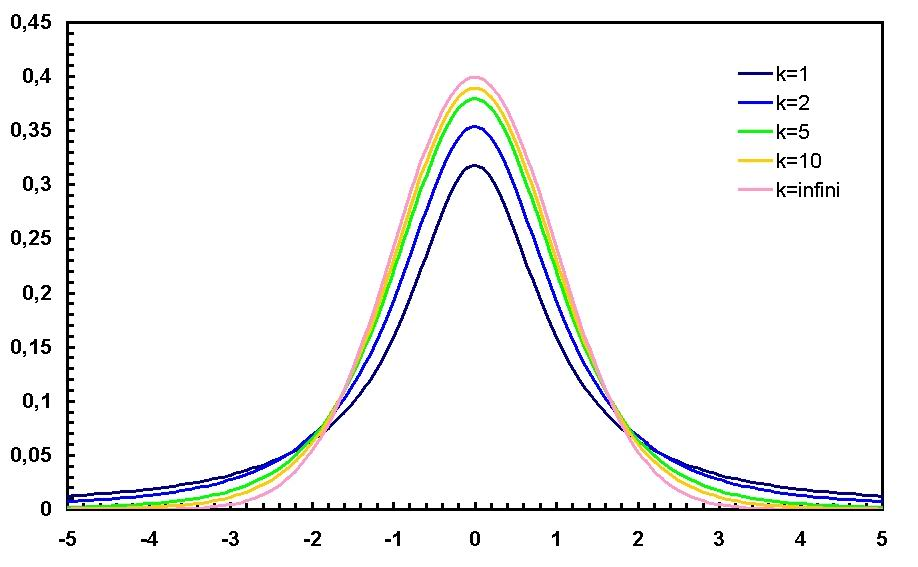
\includegraphics[width=\textwidth]{16_statystyka/tsudent.jpg}\\
\small\url{https://commons.wikimedia.org/wiki/File:Student_densite_best.JPG}
\end{frame}

\begin{frame}{Hobbici raz jeszcze}
\url{https://pl.wikisource.org/w/index.php?title=Tablica_rozk\%C5\%82adu_t-Studenta&oldid=1187619}
\begin{description}
\item[parametry] $\alpha=0{,}05$
\pause
\item[próba I] $m_{10}=3{,}21$, $\hat{s}^2_{10}=0{,}62$
\pause
\item[próba II] $m_{10}=2{,}98$, $\hat{s}^2_{10}=1{,}11$
\end{description}
\pause
\alert{Uwaga na interpretację!}
\end{frame}

\begin{frame}{}

\includegraphics[width=\textwidth]{16_statystyka/cmc20030601b.png} \\
\vfill
\small\url{http://www.theclassm.com/d/20030601.html}
\end{frame}
\end{document}
